\begin{lstlisting}[language=html]

\end{lstlisting}









\newpage

\section{LAB 2 : Indexation critériée d'observations, sélection de variables, graphiques univariés}

Dans cette deuxième session, nous allons nous intéresser à la sélection indexée d'observations ou à la restriction d'un tableau de données à un certain nombre de variables, ce qui est souvent plus pratique, soit pour faire des analyses statistiques, soit pour faire des représentations graphiques.
\subsection*{Récupération du code épuré du précédent lab}
\textbf{Note : } il existe deux possibilités pour chargé un fichier : 
\begin{enumerate}
\item Appuyer sur le bouton source sachant que le script est déjà écrit dans le workspace
\item Utiliser la fonction load pour charger des données : ex : \textit{load("smp\_lab2.rda")}
\end{enumerate}

\begin{lstlisting}[language=html]
> smp <- read.csv2("../DONNEES/smp2.csv")
> ##Affichage des variables
> names(smp)
 [1] "age"          "prof"         "duree"        "discip"       "n.enfant"     "n.fratrie"    "ecole"       
 [8] "separation"   "juge.enfant"  "place"        "abus"         "grav.cons"    "dep.cons"     "ago.cons"    
[15] "ptsd.cons"    "alc.cons"     "subst.cons"   "scz.cons"     "char"         "rs"           "ed"          
[22] "dr"           "suicide.s"    "suicide.hr"   "suicide.past" "dur.interv"  
> ##Synthèse des variables
> str(smp)
'data.frame': 799 obs. of  26 variables:
 $ age         : int  31 49 50 47 23 34 24 52 42 45 ...
 $ prof        : Factor w/ 8 levels "agriculteur",..: 3 NA 7 6 8 6 3 2 6 6 ...
 $ duree       : int  4 NA 5 NA 4 NA NA 5 4 NA ...
 $ discip      : int  0 0 0 0 1 0 0 0 1 0 ...
 $ n.enfant    : int  2 7 2 0 1 3 5 2 1 2 ...
 $ n.fratrie   : int  4 3 2 6 6 2 3 9 12 5 ...
 $ ecole       : int  1 2 2 1 1 2 1 2 1 2 ...
 $ separation  : int  0 1 0 1 1 0 1 0 1 0 ...
 $ juge.enfant : int  0 0 0 0 NA 0 1 0 1 0 ...
 $ place       : int  0 0 0 1 1 0 1 0 0 0 ...
 $ abus        : int  0 0 0 0 0 0 0 0 1 1 ...
 $ grav.cons   : int  1 2 2 1 2 1 5 1 5 5 ...
 $ dep.cons    : int  0 0 0 0 1 0 1 0 1 0 ...
 $ ago.cons    : int  1 0 0 0 0 0 0 0 0 0 ...
 $ ptsd.cons   : int  0 0 0 0 0 0 0 0 0 0 ...
 $ alc.cons    : int  0 0 0 0 0 0 0 0 1 1 ...
 $ subst.cons  : int  0 0 0 0 0 0 1 0 1 0 ...
 $ scz.cons    : int  0 0 0 0 0 0 0 0 0 0 ...
 $ char        : int  1 1 1 1 1 1 1 1 4 1 ...
 $ rs          : int  2 2 2 2 2 1 3 2 3 2 ...
 $ ed          : int  1 2 3 2 2 2 3 2 3 2 ...
 $ dr          : int  1 1 2 2 2 1 2 2 1 2 ...
 $ suicide.s   : int  0 0 0 1 0 0 3 0 4 0 ...
 $ suicide.hr  : int  0 0 0 0 0 0 1 0 1 0 ...
 $ suicide.past: int  0 0 0 0 1 0 1 0 1 0 ...
 $ dur.interv  : int  NA 70 NA 105 NA NA 105 84 78 60 ...
> ##Résumé des principaux indicateurs statistique sur les variables.
> summary(smp)
      age                       prof         duree           discip         n.enfant        n.fratrie     
 Min.   :19.0   ouvrier           :227   Min.   :1.000   Min.   :0.000   Min.   : 0.000   Min.   : 0.000  
 1st Qu.:28.0   sans emploi       :222   1st Qu.:4.000   1st Qu.:0.000   1st Qu.: 0.000   1st Qu.: 2.000  
 Median :37.0   employe           :135   Median :5.000   Median :0.000   Median : 1.000   Median : 3.000  
 Mean   :38.9   artisan           : 90   Mean   :4.302   Mean   :0.232   Mean   : 1.755   Mean   : 4.287  
 3rd Qu.:48.0   prof.intermediaire: 58   3rd Qu.:5.000   3rd Qu.:0.000   3rd Qu.: 3.000   3rd Qu.: 6.000  
 Max.   :83.0   (Other)           : 61   Max.   :5.000   Max.   :1.000   Max.   :13.000   Max.   :21.000  
 NA's   :2      NA's              :  6   NA's   :223     NA's   :6       NA's   :26                       
     ecole         separation      juge.enfant         place             abus          grav.cons    
 Min.   :1.000   Min.   :0.0000   Min.   :0.0000   Min.   :0.0000   Min.   :0.0000   Min.   :1.000  
 1st Qu.:1.000   1st Qu.:0.0000   1st Qu.:0.0000   1st Qu.:0.0000   1st Qu.:0.0000   1st Qu.:2.000  
 Median :2.000   Median :0.0000   Median :0.0000   Median :0.0000   Median :0.0000   Median :4.000  
 Mean   :1.866   Mean   :0.4226   Mean   :0.2771   Mean   :0.2285   Mean   :0.2778   Mean   :3.643  
 3rd Qu.:2.000   3rd Qu.:1.0000   3rd Qu.:1.0000   3rd Qu.:0.0000   3rd Qu.:1.0000   3rd Qu.:5.000  
 Max.   :5.000   Max.   :1.0000   Max.   :1.0000   Max.   :1.0000   Max.   :1.0000   Max.   :7.000  
 NA's   :5       NA's   :11       NA's   :5        NA's   :7        NA's   :7        NA's   :4      
    dep.cons         ago.cons        ptsd.cons         alc.cons        subst.cons        scz.cons     
 Min.   :0.0000   Min.   :0.0000   Min.   :0.0000   Min.   :0.0000   Min.   :0.0000   Min.   :0.0000  
 1st Qu.:0.0000   1st Qu.:0.0000   1st Qu.:0.0000   1st Qu.:0.0000   1st Qu.:0.0000   1st Qu.:0.0000  
 Median :0.0000   Median :0.0000   Median :0.0000   Median :0.0000   Median :0.0000   Median :0.0000  
 Mean   :0.3967   Mean   :0.1665   Mean   :0.2165   Mean   :0.1865   Mean   :0.2653   Mean   :0.0826  
 3rd Qu.:1.0000   3rd Qu.:0.0000   3rd Qu.:0.0000   3rd Qu.:0.0000   3rd Qu.:1.0000   3rd Qu.:0.0000  
 Max.   :1.0000   Max.   :1.0000   Max.   :1.0000   Max.   :1.0000   Max.   :1.0000   Max.   :1.0000  
                                                                                                      
      char             rs              ed              dr          suicide.s        suicide.hr      suicide.past   
 Min.   :1.000   Min.   :1.000   Min.   :1.000   Min.   :1.000   Min.   :0.0000   Min.   :0.0000   Min.   :0.0000  
 1st Qu.:1.000   1st Qu.:1.000   1st Qu.:1.000   1st Qu.:1.000   1st Qu.:0.0000   1st Qu.:0.0000   1st Qu.:0.0000  
 Median :1.000   Median :2.000   Median :2.000   Median :2.000   Median :0.0000   Median :0.0000   Median :0.0000  
 Mean   :1.512   Mean   :2.057   Mean   :1.866   Mean   :2.153   Mean   :0.7942   Mean   :0.2013   Mean   :0.2841  
 3rd Qu.:2.000   3rd Qu.:3.000   3rd Qu.:3.000   3rd Qu.:3.000   3rd Qu.:1.0000   3rd Qu.:0.0000   3rd Qu.:1.0000  
 Max.   :4.000   Max.   :3.000   Max.   :3.000   Max.   :3.000   Max.   :5.0000   Max.   :1.0000   Max.   :1.0000  
 NA's   :96      NA's   :103     NA's   :107     NA's   :111     NA's   :41       NA's   :39       NA's   :14      
   dur.interv    
 Min.   :  0.00  
 1st Qu.: 48.00  
 Median : 60.00  
 Mean   : 61.89  
 3rd Qu.: 75.00  
 Max.   :120.00  
 NA's   :50     

> ##Création d'une variable qualitative
> gauss <- factor(smp$n.enfant)
> levels(gauss)
 [1] "0"  "1"  "2"  "3"  "4"  "5"  "6"  "7"  "8"  "9"  "10" "11" "13"
> ##Concaténation de plusieurs mode
> levels(gauss)[6:13]<-"5+"
> levels(gauss)
[1] "0"  "1"  "2"  "3"  "4"  "5+"
> table(gauss)
gauss
  0   1   2   3   4  5+ 
214 220 125 101  55  58 

> #POUR LES VARIABLES NUMERIQUES
> ##Accès direct à des données dans une variable
> smp$age[1]
[1] 31
> ##Accès direct à des données dans un dataframe
> ### Accès à l'observation 1 de la variable 1
> names(smp)
 [1] "age"          "prof"         "duree"        "discip"       "n.enfant"     "n.fratrie"    "ecole"       
 [8] "separation"   "juge.enfant"  "place"        "abus"         "grav.cons"    "dep.cons"     "ago.cons"    
[15] "ptsd.cons"    "alc.cons"     "subst.cons"   "scz.cons"     "char"         "rs"           "ed"          
[22] "dr"           "suicide.s"    "suicide.hr"   "suicide.past" "dur.interv"  
> smp[1,1]
[1] 31
> ###OU
> smp[1,"age"]
[1] 31

> #POUR LES VARIABLES CATEGORIELLES
> table(smp$prof)

       agriculteur            artisan              autre              cadre            employe            ouvrier 
                 6                 90                 31                 24                135                227 
prof.intermediaire        sans emploi 
                58                222 
> head(smp$prof)
[1] autre              <NA>               prof.intermediaire ouvrier            sans emploi       
[6] ouvrier           
Levels: agriculteur artisan autre cadre employe ouvrier prof.intermediaire sans emploi
> ###Restriction d'une variable à une seule modalité
> table(smp$prof == "agriculteur")

FALSE  TRUE 
  787     6 
> ###Affichage des valeurs qui remplissent la condition :
> which(smp$prof =="agriculteur")
[1]  15 312 384 391 439 442
> ###Ce principe d'indexation associe à une valeur particulier, une position donnée.
> ###Ainsi, il nous est facile d'indexer les valeurs d'age pour lequelles la profession du détenu est agriculteur
> smp$age[which(smp$prof =="agriculteur")]
[1] 64 42 37 36 35 79
> ###En fait, on prend la variable age et on lui indique la liste des numéros d'obervations qui nous intéressent
> ####Conclusion : Nous avons l'age des individus dont la profession est agriculteur.

> ##Méthode plus rapide (DATAFRAME,CONDI,VARIABLE qui nous intéresse)
> subset(smp,prof=="agriculteur",age)
    age
15   64
312  42
384  37
391  36
439  35
442  79
> ##Si l'on souhaite étendre la selection à plusieurs variables :
> subset(smp,prof=="agriculteur",1:5)
    age        prof duree discip n.enfant
15   64 agriculteur    NA      0        3
312  42 agriculteur     4      0        3
384  37 agriculteur     5      1        2
391  36 agriculteur     4      1        3
439  35 agriculteur     3      0        0
442  79 agriculteur     5      0        5
> names(smp)[1:5]
[1] "age"      "prof"     "duree"    "discip"   "n.enfant"
> subset(smp,prof=="agriculteur", c(age, duree, discip,n.enfant))
    age duree discip n.enfant
15   64    NA      0        3
312  42     4      0        3
384  37     5      1        2
391  36     4      1        3
439  35     3      0        0
442  79     5      0        5
> ##La profession ne nous intéresse pas puisque nous savons déjà qu'il sont agriculteurs
> ###
> ##Il est possible de rajouter des filtres sur les lignes
> subset(smp,prof=="agriculteur" & n.enfant > 2, c(age, duree, discip,n.enfant))
    age duree discip n.enfant
15   64    NA      0        3
312  42     4      0        3
391  36     4      1        3
442  79     5      0        5
> subset(smp,prof=="agriculteur" & n.enfant > 2 & complete.cases(duree), c(age, duree, discip,n.enfant))
    age duree discip n.enfant
312  42     4      0        3
391  36     4      1        3
442  79     5      0        5
> ###

> table(gauss)
gauss
  0   1   2   3   4  5+ 
214 220 125 101  55  58 
> tab <-table(gauss)
> tab
gauss
  0   1   2   3   4  5+ 
214 220 125 101  55  58 
> sum(tab)
[1] 773
> tab/sum(tab)
gauss
         0          1          2          3          4         5+ 
0.27684347 0.28460543 0.16170763 0.13065977 0.07115136 0.07503234 
> ##R procède mode par mode [0:(214/773)=0.276...],[1:(220/773)=0.284...], ...
> ##Il existe une fonction equivalente à tab/sum(tab)
> prop.table(tab)
gauss
         0          1          2          3          4         5+ 
0.27684347 0.28460543 0.16170763 0.13065977 0.07115136 0.07503234 
> ##Arrondit des résultats :
> round(prop.table(tab),3)
gauss
    0     1     2     3     4    5+ 
0.277 0.285 0.162 0.131 0.071 0.075 
> round(prop.table(tab),2)
gauss
   0    1    2    3    4   5+ 
0.28 0.28 0.16 0.13 0.07 0.08 
> round(prop.table(tab),4)
gauss
     0      1      2      3      4     5+ 
0.2768 0.2846 0.1617 0.1307 0.0712 0.0750 

> freqrelative <- prop.table(tab)*100
> freqrelative
gauss
        0         1         2         3         4        5+ 
27.684347 28.460543 16.170763 13.065977  7.115136  7.503234 

barplot(freqrelative, xlab = "freqrelative")
\end{lstlisting}
\begin{figure}[H]\begin{center}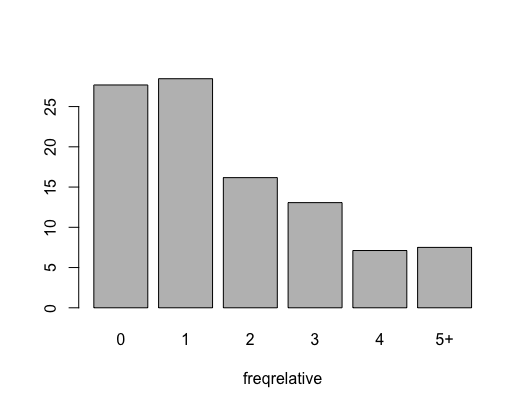
\includegraphics[scale=0.45]{ilu/lab2-1.png}\end{center}\end{figure}

\begin{lstlisting}[language=html]
barplot(freqrelative,ylim = c(0,30), xlab = "freqrelative, ylim = c(0,30)")
\end{lstlisting}
 

\begin{lstlisting}[language=html]
barplot(freqrelative,ylim = c(0,30),las=1,xlab = "freqrelative, ylim = c(0,30),las=1,xlab")
\end{lstlisting}
\begin{figure}[H]\begin{center}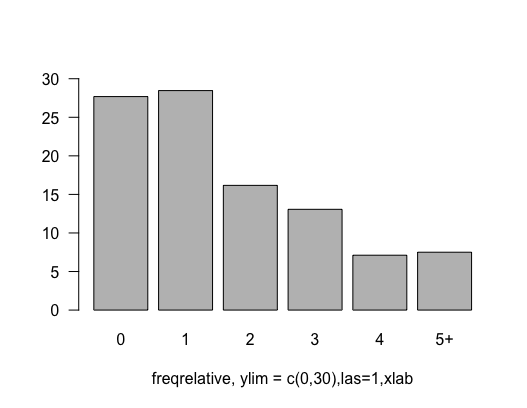
\includegraphics[scale=0.45]{ilu/lab2-3.png}\end{center}\end{figure}

\begin{lstlisting}[language=html]
> head(smp$age)
[1] 31 49 50 47 23 34
> summary(smp$age)
   Min. 1st Qu.  Median    Mean 3rd Qu.    Max.    NA's 
   19.0    28.0    37.0    38.9    48.0    83.0       2 
> ##Histogramme de Frequence
> hist(smp$age)
\end{lstlisting}

\begin{figure}[H]\begin{center}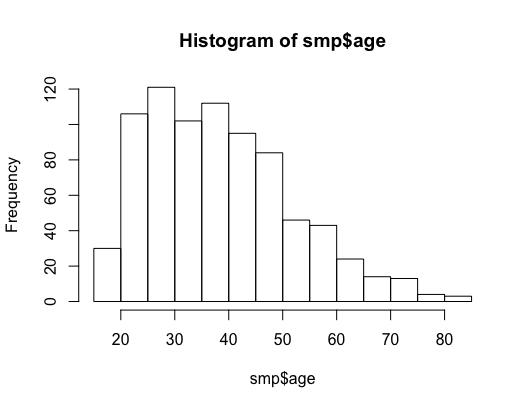
\includegraphics[scale=0.45]{ilu/lab2-4.png}\end{center}\end{figure}

\begin{lstlisting}[language=html]
lines(density(smp$age, na.rm = TRUE))
\end{lstlisting}

\begin{figure}[H]\begin{center}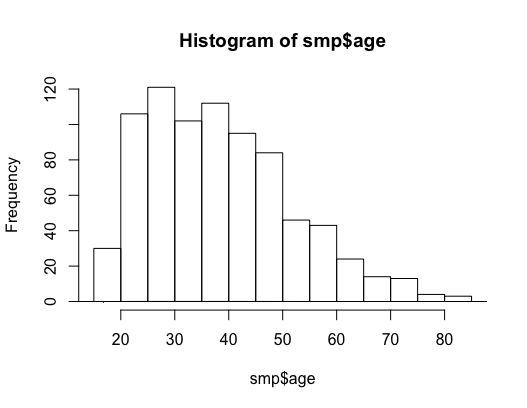
\includegraphics[scale=0.45]{ilu/lab2-5.png}\end{center}\end{figure}

\begin{lstlisting}[language=html]
> ##Conversion de l'histogramme en histogoramme de densité
> hist(smp$age,nclass = 8,prob=TRUE)
\end{lstlisting}

\begin{figure}[H]\begin{center}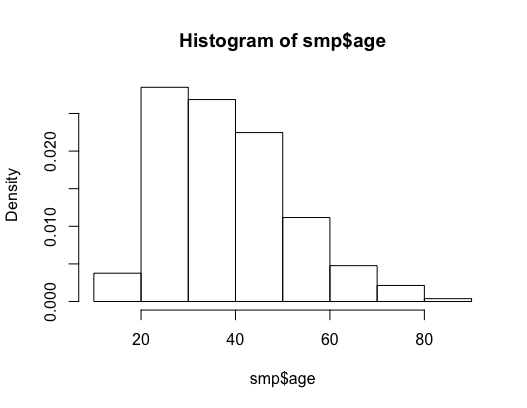
\includegraphics[scale=0.45]{ilu/lab2-6.png}\end{center}\end{figure}

\begin{lstlisting}[language=html]
> hist(smp$age,nclass = 8,prob=TRUE,las=1)
\end{lstlisting}

\begin{figure}[H]\begin{center}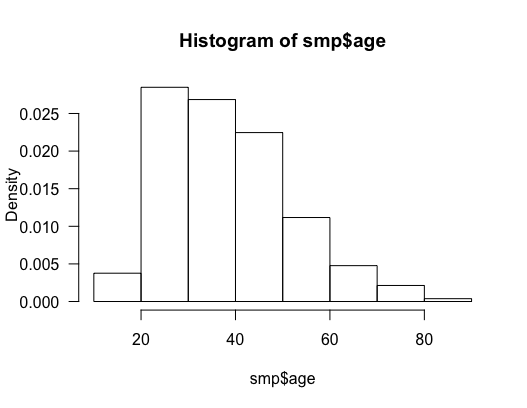
\includegraphics[scale=0.45]{ilu/lab2-7.png}\end{center}\end{figure}
\begin{lstlisting}[language=html]
lines(density(smp$age, na.rm = TRUE))
\end{lstlisting}

\begin{figure}[H]\begin{center}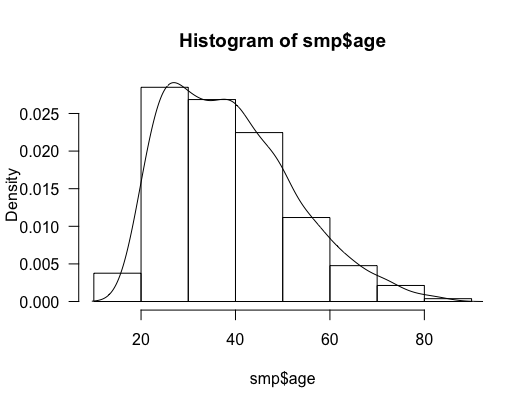
\includegraphics[scale=0.45]{ilu/lab2-8.png}\end{center}\end{figure}
\begin{lstlisting}[language=html]
##Sauvegarde du fichier de données
save(smp,file="smp_lab2.rda")
\end{lstlisting}

\newpage

\section{LAB 3 : Langage R Markdown - Génération d'un rapport automatique}

Nous avons vu à la session précédente qu'il était possible d'enregistrer toutes les commandes que l'on tape dans la console R dans un fichier de commandes ou fichier de script R, ce qui nous permet évidemment de rejouer l'analyse et facilite la reproductibilité des résultats.\newline
Nous allons voir qu'on peut également utiliser le langage R Markdown qui est un langage de formatage de documents qui permet de générer des rapports automatiques que l'on peut exporter au format HTML, au format PDF ou alors au format Microsoft Word.\newline
Rmarkdown est intégré dans Rstudio depuis les versions les plus récentes et nous n'avons plus besoin d'installer le package pour pouvoir compiler des documents au format HTML.

\begin{lstlisting}[language=html]
> setwd("~/Desktop/DIVERS_TEMPLATES/R/TP/LAB3")
> smp <- read.csv2("../DONNEES/smp2.csv")
> names(smp)
 [1] "age"          "prof"         "duree"        "discip"       "n.enfant"     "n.fratrie"    "ecole"       
 [8] "separation"   "juge.enfant"  "place"        "abus"         "grav.cons"    "dep.cons"     "ago.cons"    
[15] "ptsd.cons"    "alc.cons"     "subst.cons"   "scz.cons"     "char"         "rs"           "ed"          
[22] "dr"           "suicide.s"    "suicide.hr"   "suicide.past" "dur.interv"  
> str(smp)
'data.frame':	799 obs. of  26 variables:
 $ age         : int  31 49 50 47 23 34 24 52 42 45 ...
 $ prof        : Factor w/ 8 levels "agriculteur",..: 3 NA 7 6 8 6 3 2 6 6 ...
 $ duree       : int  4 NA 5 NA 4 NA NA 5 4 NA ...
 $ discip      : int  0 0 0 0 1 0 0 0 1 0 ...
 $ n.enfant    : int  2 7 2 0 1 3 5 2 1 2 ...
 $ n.fratrie   : int  4 3 2 6 6 2 3 9 12 5 ...
 $ ecole       : int  1 2 2 1 1 2 1 2 1 2 ...
 $ separation  : int  0 1 0 1 1 0 1 0 1 0 ...
 $ juge.enfant : int  0 0 0 0 NA 0 1 0 1 0 ...
 $ place       : int  0 0 0 1 1 0 1 0 0 0 ...
 $ abus        : int  0 0 0 0 0 0 0 0 1 1 ...
 $ grav.cons   : int  1 2 2 1 2 1 5 1 5 5 ...
 $ dep.cons    : int  0 0 0 0 1 0 1 0 1 0 ...
 $ ago.cons    : int  1 0 0 0 0 0 0 0 0 0 ...
 $ ptsd.cons   : int  0 0 0 0 0 0 0 0 0 0 ...
 $ alc.cons    : int  0 0 0 0 0 0 0 0 1 1 ...
 $ subst.cons  : int  0 0 0 0 0 0 1 0 1 0 ...
 $ scz.cons    : int  0 0 0 0 0 0 0 0 0 0 ...
 $ char        : int  1 1 1 1 1 1 1 1 4 1 ...
 $ rs          : int  2 2 2 2 2 1 3 2 3 2 ...
 $ ed          : int  1 2 3 2 2 2 3 2 3 2 ...
 $ dr          : int  1 1 2 2 2 1 2 2 1 2 ...
 $ suicide.s   : int  0 0 0 1 0 0 3 0 4 0 ...
 $ suicide.hr  : int  0 0 0 0 0 0 1 0 1 0 ...
 $ suicide.past: int  0 0 0 0 1 0 1 0 1 0 ...
 $ dur.interv  : int  NA 70 NA 105 NA NA 105 84 78 60 ...
> summary(smp)
      age                       prof         duree           discip         n.enfant        n.fratrie     
 Min.   :19.0   ouvrier           :227   Min.   :1.000   Min.   :0.000   Min.   : 0.000   Min.   : 0.000  
 1st Qu.:28.0   sans emploi       :222   1st Qu.:4.000   1st Qu.:0.000   1st Qu.: 0.000   1st Qu.: 2.000  
 Median :37.0   employe           :135   Median :5.000   Median :0.000   Median : 1.000   Median : 3.000  
 Mean   :38.9   artisan           : 90   Mean   :4.302   Mean   :0.232   Mean   : 1.755   Mean   : 4.287  
 3rd Qu.:48.0   prof.intermediaire: 58   3rd Qu.:5.000   3rd Qu.:0.000   3rd Qu.: 3.000   3rd Qu.: 6.000  
 Max.   :83.0   (Other)           : 61   Max.   :5.000   Max.   :1.000   Max.   :13.000   Max.   :21.000  
 NA's   :2      NA's              :  6   NA's   :223     NA's   :6       NA's   :26                       
     ecole         separation      juge.enfant         place             abus          grav.cons    
 Min.   :1.000   Min.   :0.0000   Min.   :0.0000   Min.   :0.0000   Min.   :0.0000   Min.   :1.000  
 1st Qu.:1.000   1st Qu.:0.0000   1st Qu.:0.0000   1st Qu.:0.0000   1st Qu.:0.0000   1st Qu.:2.000  
 Median :2.000   Median :0.0000   Median :0.0000   Median :0.0000   Median :0.0000   Median :4.000  
 Mean   :1.866   Mean   :0.4226   Mean   :0.2771   Mean   :0.2285   Mean   :0.2778   Mean   :3.643  
 3rd Qu.:2.000   3rd Qu.:1.0000   3rd Qu.:1.0000   3rd Qu.:0.0000   3rd Qu.:1.0000   3rd Qu.:5.000  
 Max.   :5.000   Max.   :1.0000   Max.   :1.0000   Max.   :1.0000   Max.   :1.0000   Max.   :7.000  
 NA's   :5       NA's   :11       NA's   :5        NA's   :7        NA's   :7        NA's   :4      
    dep.cons         ago.cons        ptsd.cons         alc.cons        subst.cons        scz.cons     
 Min.   :0.0000   Min.   :0.0000   Min.   :0.0000   Min.   :0.0000   Min.   :0.0000   Min.   :0.0000  
 1st Qu.:0.0000   1st Qu.:0.0000   1st Qu.:0.0000   1st Qu.:0.0000   1st Qu.:0.0000   1st Qu.:0.0000  
 Median :0.0000   Median :0.0000   Median :0.0000   Median :0.0000   Median :0.0000   Median :0.0000  
 Mean   :0.3967   Mean   :0.1665   Mean   :0.2165   Mean   :0.1865   Mean   :0.2653   Mean   :0.0826  
 3rd Qu.:1.0000   3rd Qu.:0.0000   3rd Qu.:0.0000   3rd Qu.:0.0000   3rd Qu.:1.0000   3rd Qu.:0.0000  
 Max.   :1.0000   Max.   :1.0000   Max.   :1.0000   Max.   :1.0000   Max.   :1.0000   Max.   :1.0000  
                                                                                                      
      char             rs              ed              dr          suicide.s        suicide.hr      suicide.past   
 Min.   :1.000   Min.   :1.000   Min.   :1.000   Min.   :1.000   Min.   :0.0000   Min.   :0.0000   Min.   :0.0000  
 1st Qu.:1.000   1st Qu.:1.000   1st Qu.:1.000   1st Qu.:1.000   1st Qu.:0.0000   1st Qu.:0.0000   1st Qu.:0.0000  
 Median :1.000   Median :2.000   Median :2.000   Median :2.000   Median :0.0000   Median :0.0000   Median :0.0000  
 Mean   :1.512   Mean   :2.057   Mean   :1.866   Mean   :2.153   Mean   :0.7942   Mean   :0.2013   Mean   :0.2841  
 3rd Qu.:2.000   3rd Qu.:3.000   3rd Qu.:3.000   3rd Qu.:3.000   3rd Qu.:1.0000   3rd Qu.:0.0000   3rd Qu.:1.0000  
 Max.   :4.000   Max.   :3.000   Max.   :3.000   Max.   :3.000   Max.   :5.0000   Max.   :1.0000   Max.   :1.0000  
 NA's   :96      NA's   :103     NA's   :107     NA's   :111     NA's   :41       NA's   :39       NA's   :14      
   dur.interv    
 Min.   :  0.00  
 1st Qu.: 48.00  
 Median : 60.00  
 Mean   : 61.89  
 3rd Qu.: 75.00  
 Max.   :120.00  
 NA's   :50      
> gauss <- factor(smp$n.enfant)
> table(gauss)
gauss
  0   1   2   3   4   5   6   7   8   9  10  11  13 
214 220 125 101  55  31   7   7   7   2   2   1   1 
> levels(gauss)[6:13]<-"5+"
> table(gauss)
gauss
  0   1   2   3   4  5+ 
214 220 125 101  55  58 
> f <- prop.table(table(gauss))*100
> r<-sum(f)/100
> f
gauss
        0         1         2         3         4        5+ 
27.684347 28.460543 16.170763 13.065977  7.115136  7.503234 
> ##"La somme cumulée des fréquence est :")
> r
[1] 1
> barplot(f, ylim = c(0,30),las=1)
\end{lstlisting}

\begin{figure}[H]\begin{center}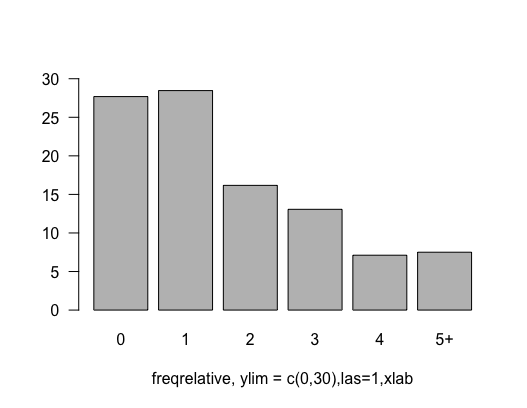
\includegraphics[scale=0.45]{ilu/lab2-3.png}\end{center}\end{figure}

Nous allons à présent générer un autre document : le RMarkdown\newline
Il faut donc installer les packages \textit{markdown} et \textit{rmarkdown} sur le site du CRAN ou directement via RSTUDIO.\newline

\begin{figure}[H]\begin{center}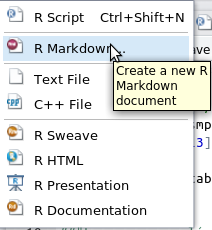
\includegraphics[scale=0.5]{ilu/bz.png}\end{center}\end{figure}

Nous pouvons voir (sur la figure ci dessous qu'il existe plusieurs formats possibles). Nous allons choisir le premier : \textit{Document} et la sortie au format \textit{HTML}

Une fois les champs Titres et Auteurs remplies, R va générer un document standard pour la sortie choisie.\newline
Il est toujours possible de modifier de langage pour l'output : 

\begin{figure}[H]\begin{center}
\includegraphics[scale=0.5]{ilu/cb.png}\end{center}\end{figure} 

Nous rajoutons un phrase d'introduction et nous cliquons sur \textit{Chunks/Insert Chunks} qui signifie à RSTUDIO qu'il faut évaluer les lignes de codes présent entre les accolades : 
\begin{lstlisting}[language=html]
---
title: "Exemple_d_analse"
author: "LATIF Mehdi"
date: "11/10/2016"
output: html_document
---
#Analyse des données sur la santé mentale en prison : 
```{r}

```
\end{lstlisting}

Nous allons alors compléter le code markdown : 

\begin{lstlisting}[language=html]
---
title: "Exemple d'analyse"
author: "LATIF Mehdi"
date: "11/10/2016"
output: html_document
---
## Description : Analyse des données sur la santé mentale en prison : 

**URL** : http://rmarkdown.rstudio.com/authoring_basics.html

Défintion du workspace par défaut et chargement du dataframe
```{r}
setwd("~/XX_Université_fun/univfunR/TP/LAB3")
smp <- read.csv2("/comptes/E131729J/XX_Université_fun/univfunR/TP/smp2.csv")
```
######TADAH
**Note :**  Si l'on considère que ce n'est pas important à affichier, il suffit d'écrire dans le chunk echo = FALSE
```{r echo=FALSE}
setwd("~/XX_Université_fun/univfunR/TP/LAB3")
smp <- read.csv2("/comptes/E131729J/XX_Université_fun/univfunR/TP/smp2.csv")
```
######Et rien apparait RETADAH

Affichage des variables contenues dans le DATAFRAMES SMP
```{r}
names(smp)
```
Résumé synthétique des différentes variables contenues dans le fichier SMP
```{r}
str(smp)
```
Affichage des principaux paramètres statistiques des différentes variables contenues dans le fichier SMP
variables contenues dans le fichier SMP
```{r}
summary(smp)
```
**Note :** Il est possible de faire un affichage unique de trois commandes dans un même _chunk_ : pour cela, il faut ecrire : 
_{r, eval = c(1,3)}_ (Dans notre cas, les lignes que l'on souhaites évaluer sont les lignes de commandes 1 et 3) :
```{r, eval = c(1,3)}
names(smp)
str(smp)
summary(smp)
```
Définition d'une nouvelle variable _gauss_, variable catégorielle (on dit aussi qualitative) ou **l'âge des enfants est une modalité**
```{r}
gauss <- factor(smp$n.enfant)
table(gauss)
```
Redéfinition d'une modalité dans la variable catégoricielle _gauss_. On concatène les âges supérieurs à 6 ans et on les rassemble dans une même modalité : 
```{r}
levels(gauss)[6:13]<-"5+"
table(gauss)
```
Affichage des pourcentage de chaque modalité de la variable : 
```{r}
prop.table(table(gauss))
```
Modification des pourcentage (x100) pour avoir des résultats plus _lisibles_ : 
```{r}
f <- prop.table(table(gauss))*100
f
```
**Vérification :** La somme des fréquences cumulée est bien égale à 1 :
```{r}
r<-sum(f)/100
r
```
**Représentation graphique** sous forme d'histogramme de la variable qualitative _gauss_
```{r}
barplot(f, ylim = c(0,30),las=1,xlab="catégorie d'âge", ylab="Population")
```
\end{lstlisting}

Compilons ce code dans un fichier markdown et c'est magique.
%\input{first_markdown.html}
\newpage

\section{LAB 4 : Tests d'associations et graphiques bivariés}

Dans la session précédente, nous avons vu comment manipuler un dataframe, les variables contenues dans ce dernier et que l'on pouvait produire des résumés numériques pour des variables numériques ou qualitatives ainsi que des graphiques élémentaires à l'aide du langage RMarkdown.\newline
Nous allons cette fois ci nous intéresser au croisement de deux variables, soit qualitatives, c'est à dire un \textbf{tableau de contigence}, soit une variable qualitative et une numérique ce qui donnera lieu à la comparaison de deux moyennes.\newline

On rappelle que l'on peut charger directement un fichier de données à l'aide de la commande \textit{load()}.

\begin{lstlisting}[language=html]
> setwd("~/Desktop/DIVERS_TEMPLATES/R/TP/LAB4")
> load("~/Desktop/DIVERS_TEMPLATES/R/TP/smp_v1.rda")
\end{lstlisting}
Nous retrouvons bien notre dataframe avec 799 observations et 27 variables.

\begin{figure}[H]\begin{center}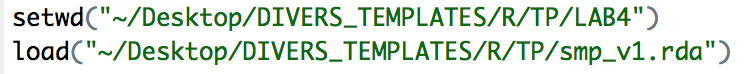
\includegraphics[scale=0.6]{ilu/cf.png}\\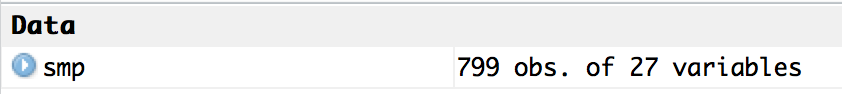
\includegraphics[scale=0.6]{ilu/cg.png}\end{center}\end{figure}
Nous pouvons afficher un tableau d'effectif simple pour la variable consommation de substance : 
\begin{lstlisting}[language=html]
> table(smp$subst.cons)

  0   1 
587 212 
> table(smp$subst.cons,useNA = "always")

   0    1 <NA> 
 587  212    0 
\end{lstlisting}

On peut également croisé cette dernière avec la variable abus qui est une variable binaire :
\begin{lstlisting}[language=html]
> table(smp$subst.cons, smp$abus)
   
      0   1
  0 441 140
  1 131  80
> tab <- table(smp$subst.cons, smp$abus)
> tab
   
      0   1
  0 441 140
  1 131  80
\end{lstlisting}

On obtient donc un tableau de contingence avec les modalités de la première variables qui apparaissent en ligne et celles de la seconde variable qui apparaissent en colonne (ici, 0 ou 1).\newline
\\ 
On peut également calculer les fréquence grâce à la fonction \textit{prop.table()}. Il nous est également possible de spécifier sur quelle ligne ou colonne nous souhaitons calculer les fréquence avec :
\begin{itemize}
\item \textit{margin = 1} tous les effectifs vont être rapportés aux totaux lignes, donc ici $0.76$ correspondra à 441 rapporté à l'ensemble des individus qui remplissent la modalité $0$ de la variable \textit{subst.cons}, donc l'effectif ligne
\item \textit{margin = 2} tous les effectifs vont être rapportés aux totaux colonnes, donc ici 0.77 correspond ici à 441 rapporté à l'effectif total pour cette première colonne. 
\end{itemize}
\begin{lstlisting}[language=html]
> ##margin = 1 -> tous les effectifs vont être rapportés aux totaux lignes
> prop.table(tab, margin = 1)
   
            0         1
  0 0.7590361 0.2409639
  1 0.6208531 0.3791469
> ##margin = 2 -> tous les effectifs vont être rapportés aux totaux colonnes
> prop.table(tab, margin = 2)
   
            0         1
  0 0.7709790 0.6363636
  1 0.2290210 0.3636364
\end{lstlisting}
Plutôt que d'utiliser \textit{table()}, nous pouvons également utiliser la commande \textit{xtabs()} et qui présente l'avantage de fonctionner avec des formules dont on fera un plus large usage lorsque nous effectuerons des tests et pour les modèles.\newline
Nous utilisons tilde ($\sim$) pour dénoter la relation entre deux variables. Ici c'est une relation qui est complètement symétrique donc les deux variables jouent le même rôle.
\begin{lstlisting}[language=html]
> xtabs(~subst.cons + abus, smp )
          abus
subst.cons   0   1
         0 441 140
         1 131  80
\end{lstlisting}
Il est possible de représenter graphiquement les tableaux de contingence, La seule différence est qu'ici, par défaut, \textbf{R} va superposer les modalités : 

\begin{lstlisting}[language=html]
tob<-xtabs(~subst.cons + abus, smp )
barplot(tob)
\end{lstlisting}
\begin{figure}[H]\begin{center}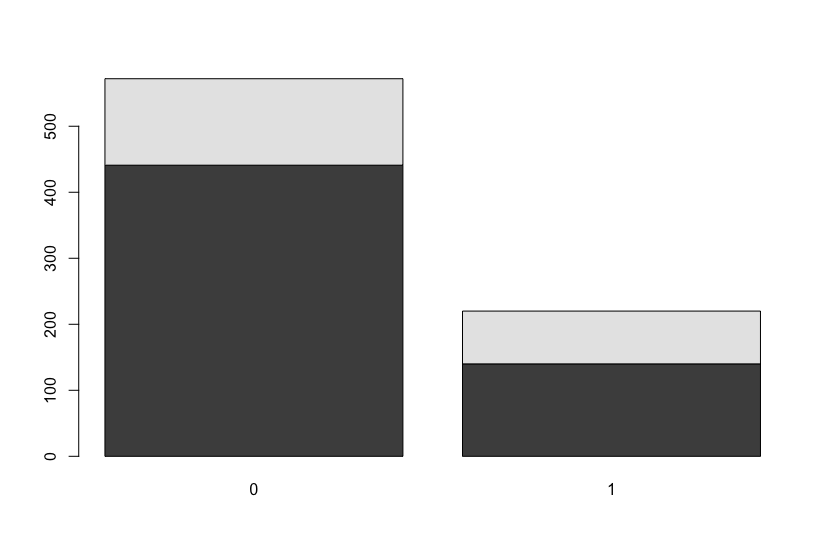
\includegraphics[scale=0.5]{ilu/ch.png}\end{center}\end{figure}
Pour afficher les modalités côte à côte, on utilise l'attribut \textit{beside = TRUE} :
\begin{lstlisting}[language=html]
barplot(tob,beside = TRUE, xlab="Modalités : Consommation de substance et Abus", ylab = "Effectifs")
\end{lstlisting}
\begin{figure}[H]\begin{center}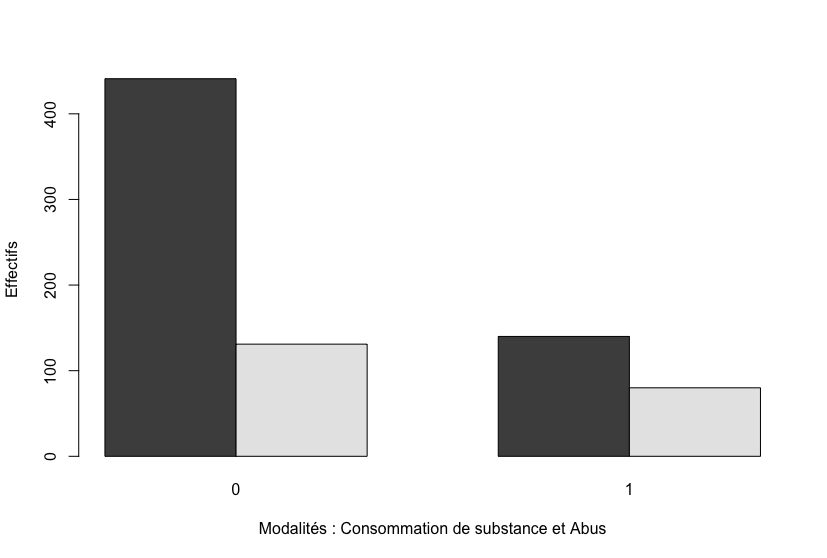
\includegraphics[scale=0.5]{ilu/ci.png}\end{center}\end{figure}
Pour réaliser un test du $\chi^{2}$, on utilise la méthode \textit{chisq.test()} qui par défaut, inclut une correction de continuité: 
\begin{lstlisting}[language=html]
> tab
   
      0   1
  0 441 140
  1 131  80
> chisq.test(tab)

	Pearson's Chi-squared test with Yates' continuity correction

data:  tab
X-squared = 14.052, df = 1, p-value = 0.0001779

> res <- chisq.test(tab)
> res

	Pearson's Chi-squared test with Yates' continuity correction

data:  tab
X-squared = 14.052, df = 1, p-value = 0.0001779

> ##Retourne le nom de la variable étudiée
> res$data.name
[1] "tab"
> ##Retourne la méthode utilisée pour le test
> res$method
[1] "Pearson's Chi-squared test with Yates' continuity correction"
> ##Retourne le résultat statistique du test
> res$statistic
X-squared 
  14.0517 
> ##Retourne le degré de liberté
> res$parameter
df 
 1 
> ##Retourne le résultat du test p-value
> res$p.value
[1] 0.0001778528
> ##Retourne le tableau de contingence sur lequel nous avons effectuée le test
> res$observed
   
      0   1
  0 441 140
  1 131  80
> ##Retourne le tableau de contingence théorique que nous devrions obtenir
> ###Effectifs attendus sous l'hypothèse d'indépendance
> res$expected
   
           0         1
  0 419.6111 161.38889
  1 152.3889  58.61111
\end{lstlisting}

Si l'on souhaite réaliser un test de \textbf{Fisher}, on utilisera la fonction \textit{fisher.test()}

\begin{lstlisting}[language=html]
> tab
   
      0   1
  0 441 140
  1 131  80
> fisher.test(tab)

	Fisher's Exact Test for Count Data

data:  tab
p-value = 0.0002193
alternative hypothesis: true odds ratio is not equal to 1
95 percent confidence interval:
 1.351339 2.728231
sample estimates:
odds ratio 
  1.921985 
\end{lstlisting}

Considérons maintenant la variable âge et nous allons chercher à décrire l'âge en fonction de la variable correspondant à la consommation de substance (subst.cons)\newline
Premièrement, nous allons afficher les modalités de la variable d'âge et le tableau d'effectif de subst.cons (ne pas oublier d'afficher au cas où, les valeurs non renseignées) :

\begin{lstlisting}[language=html]
 > head(smp$age)
[1] 31 49 50 47 23 34
> table(smp$subst.cons)

  0   1 
587 212 
> table(smp$subst.cons, useNA = "always")

   0    1 <NA> 
 587  212    0 
\end{lstlisting}

Ce qui va nous intéresser maintenant, c'est de décrire la variable âge en fonction des deux modalité de la variable consommation de substance,  0 ou 1, c'est-à-dire oui il y a consommation ou non il n'y a pas consommation; Cela revient à calculer des moyennes conditionnelles.\newline
Pour se faire, nous allons pouvoir utiliser la fonction \textit{tapply()}. Nous allons indiquer en paramètre le nom de la variable numérique que l'on souhaite caractériser (age), le nom de la variable catégorielle (subst.cons), ou critère de classification, et la commande que l'on souhaite utiliser.
\begin{lstlisting}[language=html]
> tapply(smp$age, smp$subst.cons, mean)
 0  1 
NA NA 
\end{lstlisting}
On voit ici que \textbf{R} nous renvoi les valeurs manquantes; Cela signifie qu'il existe des valeurs manquantes pour la variable age. On doit donc dire au logiciel de supprimer ces valeurs à l'aide de la fonction \textit{na.rm = TRUE}
\begin{lstlisting}[language=html]
> tapply(smp$age, smp$subst.cons, mean,na.rm = TRUE)
       0        1 
41.97099 30.36967 
\end{lstlisting}
On obtient donc la moyenne de l'âge pour les détenus ne consommant pas de substance ($41,97099$) et celle pour ceux qui en consomment ($30,36967$).\newline
\\
Pour réaliser un test de Student, nous allons utiliser la commande \textit{t.test()} en y indiquant les deux échantillons que l'on souhaite comparer. Dans notre cas, on souhaite étudier les âges pour lesquels il y a consommation de substance (\textit{smp\$age[smp\$subst.cons == 0]}) et ceux pour lesquels il n'y a pas de consommation de substance (\textit{smp\$age[smp\$subst.cons == 1]}).

\begin{lstlisting}[language=html]
> t.test(smp$age[smp$subst.cons == 0],smp$age[smp$subst.cons == 1])

	Welch Two Sample t-test

data:  smp$age[smp$subst.cons == 0] and smp$age[smp$subst.cons == 1]
t = 15.24, df = 666.83, p-value < 2.2e-16
alternative hypothesis: true difference in means is not equal to 0
95 percent confidence interval:
 10.10664 13.09600
sample estimates:
mean of x mean of y 
 41.97099  30.36967 
\end{lstlisting}

On remarque que \textbf{R} n'effectue pas directement le test de Student mais une variante de ce dernier, le test de Welsh, qui comme nous l'avons expliquer dans le cours, ne nécessite pas l'égalité des variances comme condition de validité.\newline 
Si nous souhaitons réaliser un vrai test de Student, nous devons spécifier l'égalité des variances de la manière suivante : 
\begin{lstlisting}[language=html]
> t.test(smp$age[smp$subst.cons == 0],smp$age[smp$subst.cons == 1],var.equal = TRUE)

	Two Sample t-test

data:  smp$age[smp$subst.cons == 0] and smp$age[smp$subst.cons == 1]
t = 11.785, df = 795, p-value < 2.2e-16
alternative hypothesis: true difference in means is not equal to 0
95 percent confidence interval:
  9.668959 13.533684
sample estimates:
mean of x mean of y 
 41.97099  30.36967 
\end{lstlisting}

Précédemment, nous avons vu que la fonction \textit{xtabs()} nous permettait d'utiliser une notation par formule ce qui est assez pratique puisque cela nous permet de décrire la relation entre plusieurs variables à l'aide d'une formule :

\begin{lstlisting}[language=html]
> xtabs(age~subst.cons,smp)
subst.cons
    0     1 
24595  6408 
\end{lstlisting}

Dans notre cas, les variables jouent un rôle \textbf{asymétrique} : Nous avons une \textit{variable réponse}, c'est à dire une variable dépendante : l'âge et une \textit{variable explicative} : la consommation de substances.\newline
L'objectif est donc d'écrire une relation permettant d'\textit{expliquer l'âge en fonction de la consommation de substances}.\newline
\textbf{Note :} On rappelle que le paramètre smp dans un test permet d'indiquer le data frame dans lequel se trouvent les variables.

\begin{lstlisting}[language=html]
> ##L'âge expliqué par la variable subst.cons
> t.test(age~subst.cons,smp)

	Welch Two Sample t-test

data:  age by subst.cons
t = 15.24, df = 666.83, p-value < 2.2e-16
alternative hypothesis: true difference in means is not equal to 0
95 percent confidence interval:
 10.10664 13.09600
sample estimates:
mean in group 0 mean in group 1 
       41.97099        30.36967 

> xtabs(age~subst.cons,smp)
subst.cons
    0     1 
24595  6408 
\end{lstlisting}

Nous pouvons donc remarquer que nous obtenons les mêmes résultats qu'avec le test de Student réalisé plus haut, moyennant le fait que nous ne sommes plus obligés de préfixer les variables par le nom du dataframe.\newline
\\
Nous avons vu qu'il nous était possible de calculer des moyennes conditionnelles à l'aide de la commande \textit{t.apply()}. Si l'on souhaite effectuer ce calcul tout en conservant un attribut sous forme d'une formule, nous pouvons utiliser la commande \textit{aggregate()} avec comme paramètre, la formule que l'on a définit précédemment pour les variables asymétriques. On doit cependant spécifier en attribut, la valeur que l'on souhaite calculer : ici, la moyenne (\textit{mean}).

\begin{lstlisting}[language=html]
> aggregate(age ~ subst.cons, smp, mean)
  subst.cons      age
1          0 41.97099
2          1 30.36967
\end{lstlisting}

\textbf{Note : } Contrairement à la fonction \textit{t.apply()}, dans \textit{aggregate()}, nous n'avons pas besoin pas besoin de spécifier que l'on souhaite supprimer les valeurs manquantes (\textit{na.rm = TRUE}) car cette commande est activée par défaut.\newline\\
Enfin, un autre avantage de la fonction \textit{aggregate()} est qu'elle nous renvoie directement un dataframe que l'on peut réutiliser pour réaliser des graphiques :

\begin{lstlisting}[language=html]
> ag <- aggregate(age ~ subst.cons, smp, mean)
> boxplot(ag) 
\end{lstlisting}

\begin{figure}[H]\begin{center}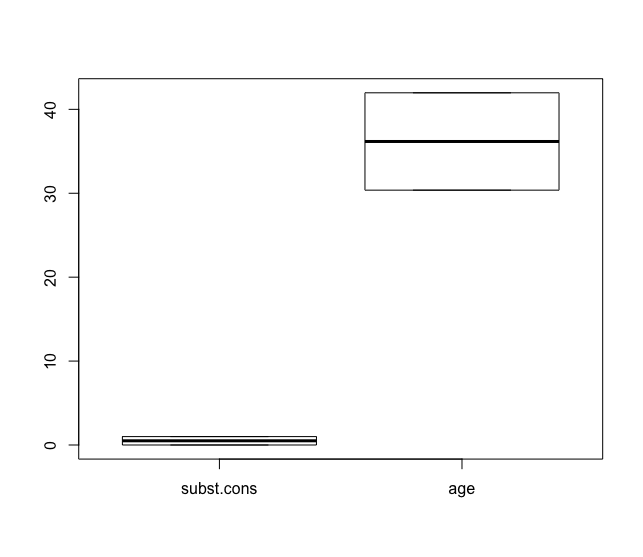
\includegraphics[scale=0.5]{ilu/cj.png}\end{center}\end{figure}

Si l'on souhaite générer une représentation graphique des distributions conditionnelles, il est encore une fois possible d'utiliser la notation par formule dans la fonction \textit{boxplot()} : 
\begin{lstlisting}[language=html]
> boxplot(age~subst.cons,smp)
\end{lstlisting}

\begin{figure}[H]\begin{center}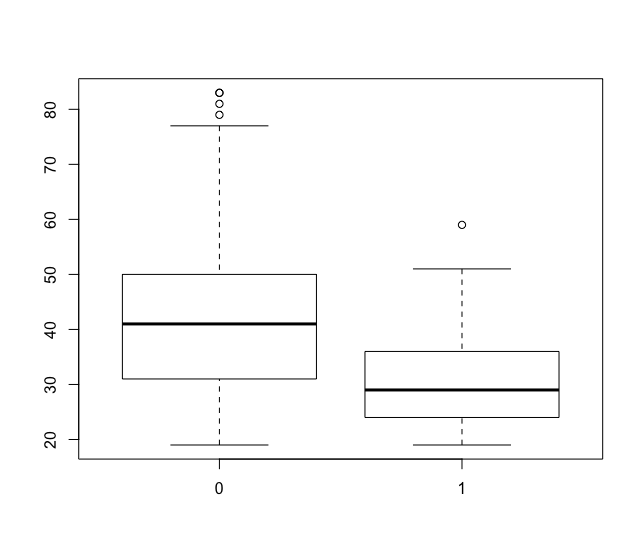
\includegraphics[scale=0.5]{ilu/ck.png}\end{center}\end{figure}

Cette fois-ci, nous obtenons une représentation en forme de boites à moustaches pour chacune des modalités de la variable \textit{subst.cons} avec en ordonnée, les valeurs prises par la variable \textit{age}.\newline
\\
\textbf{Note : } Il existe beaucoup d'autres commandes qui peuvent nous permettre de réaliser des graphiques plus élaborer. Nous les présenterons plus tard dans le cadre de la retranscription du \textit{MEETUP R}.


\newpage

\section{LAB 5 : ANOVA, Régression linéaire et logistique}
\begin{lstlisting}[language=html]
> ##Défintion du des Workspaces
> setwd("~/Desktop/DIVERS_TEMPLATES/R/TP/LAB5")
> ##Chargement des données du fichier smp
> smp <- read.csv2("../DONNEES/smpc.csv")
> ### Autre possiblité pour charger directement un fichier avec l'historique des modification :
> #load("~/Desktop/DIVERS_TEMPLATES/R/TP/smp_v1.rda")
> ##Affichage des données du Data Frame
> str(smp)
'data.frame': 799 obs. of  9 variables:
 $ age      : int  31 49 50 47 23 34 24 52 42 45 ...
 $ prof     : Factor w/ 8 levels "agriculteur",..: 3 NA 7 6 8 6 3 2 6 6 ...
 $ dep.cons : int  0 0 0 0 1 0 1 0 1 0 ...
 $ scz.cons : int  0 0 0 0 0 0 0 0 0 0 ...
 $ grav.cons: int  1 2 2 1 2 1 5 1 5 5 ...
 $ n.enfant : int  2 7 2 0 1 3 5 2 1 2 ...
 $ rs       : int  2 2 2 2 2 1 3 2 3 2 ...
 $ ed       : int  1 2 3 2 2 2 3 2 3 2 ...
 $ dr       : int  1 1 2 2 2 1 2 2 1 2 ...
> ##Affichage du résumé des données du Data Frame
> summary(smp)
      age                       prof        dep.cons         scz.cons        grav.cons        n.enfant     
 Min.   :19.0   ouvrier           :227   Min.   :0.0000   Min.   :0.0000   Min.   :1.000   Min.   : 0.000  
 1st Qu.:28.0   sans emploi       :222   1st Qu.:0.0000   1st Qu.:0.0000   1st Qu.:2.000   1st Qu.: 0.000  
 Median :37.0   employe           :135   Median :0.0000   Median :0.0000   Median :4.000   Median : 1.000  
 Mean   :38.9   artisan           : 90   Mean   :0.3967   Mean   :0.0826   Mean   :3.643   Mean   : 1.755  
 3rd Qu.:48.0   prof.intermediaire: 58   3rd Qu.:1.0000   3rd Qu.:0.0000   3rd Qu.:5.000   3rd Qu.: 3.000  
 Max.   :83.0   (Other)           : 61   Max.   :1.0000   Max.   :1.0000   Max.   :7.000   Max.   :13.000  
 NA's   :2      NA's              :  6                                     NA's   :4       NA's   :26      
       rs              ed              dr       
 Min.   :1.000   Min.   :1.000   Min.   :1.000  
 1st Qu.:1.000   1st Qu.:1.000   1st Qu.:1.000  
 Median :2.000   Median :2.000   Median :2.000  
 Mean   :2.057   Mean   :1.866   Mean   :2.153  
 3rd Qu.:3.000   3rd Qu.:3.000   3rd Qu.:3.000  
 Max.   :3.000   Max.   :3.000   Max.   :3.000  
 NA's   :103     NA's   :107     NA's   :111    
> ###############################################
> ##Nous allons nous intéresser à un sous ensemble du Data Frame smp
> ##Nous allons regarder pour les individus dont la profession est [ss-emploi & cadre & profession intermédiaire], l'âge et le nombre d'enfant :
> ###Note : | est le OU logique dans R
> ##Les Premières lignes
> head(subset(smp, prof == "sans emploi" | prof == "prof.intermediaire" | prof == "cadre", c(age,n.enfant,prof)))
   age n.enfant               prof
3   50        2 prof.intermediaire
5   23        1        sans emploi
11  31        0 prof.intermediaire
17  60        2 prof.intermediaire
23  32        0        sans emploi
27  32        1        sans emploi
> ##Autre écriture
> head(subset(smp, prof %in% c("sans emploi", "prof.intermediaire", "cadre"), c(age, n.enfant, prof)))
   age n.enfant               prof
3   50        2 prof.intermediaire
5   23        1        sans emploi
11  31        0 prof.intermediaire
17  60        2 prof.intermediaire
23  32        0        sans emploi
27  32        1        sans emploi
> ##L'ensemble des observations :
> subset(smp, prof == "sans emploi" | prof == "prof.intermediaire" | prof == "cadre", c(age,n.enfant,prof))
    age n.enfant               prof
3    50        2 prof.intermediaire
5    23        1        sans emploi
[...]
784  56        2        sans emploi
788  68        7        sans emploi
789  42        2        sans emploi
792  26        1        sans emploi
794  27        2 prof.intermediaire
795  28        1        sans emploi
797  31        3              cadre
> ## Sauvegarde dans un objet :
> smpb <- subset(smp, prof == "sans emploi" | prof == "prof.intermediaire" | prof == "cadre", c(age,n.enfant,prof))
> ## On a maintenant : smp (799 obs. of 27 variables) et smpb (246 obs. of 3 variables)
> summary(smpb)
      age           n.enfant                      prof    
 Min.   :19.00   Min.   : 0.000   sans emploi       :222  
 1st Qu.:27.00   1st Qu.: 0.000   prof.intermediaire: 58  
 Median :36.00   Median : 1.000   cadre             : 24  
 Mean   :38.42   Mean   : 1.648   agriculteur       :  0  
 3rd Qu.:47.25   3rd Qu.: 3.000   artisan           :  0  
 Max.   :83.00   Max.   :13.000   autre             :  0  
                 NA's   :11       (Other)           :  0  
> ##On remarque que pour la variable smpb.prof, R à conservé les anciens niveaux qui n'ont plus lieu d'être ici
> ## On va donc appliquer la fonction factor pour que R recalcule les niveaux de la variable
> smpb$prof <- factor(smpb$prof)
> summary(smpb)
      age           n.enfant                      prof    
 Min.   :19.00   Min.   : 0.000   cadre             : 24  
 1st Qu.:27.00   1st Qu.: 0.000   prof.intermediaire: 58  
 Median :36.00   Median : 1.000   sans emploi       :222  
 Mean   :38.42   Mean   : 1.648                           
 3rd Qu.:47.25   3rd Qu.: 3.000                           
 Max.   :83.00   Max.   :13.000                           
                 NA's   :11                               
> ##NE PAS CALCULER CE FACTEUR CAR CELA TRANSFORME UNE VARIABLE QUANTITATIVE EN VARIABLE QUALITATIVEsmpb$age <- factor(smpb$age)
> ##NE PAS CALCULER CE FACTEUR CAR CELA TRANSFORME UNE VARIABLE QUANTITATIVE EN VARIABLE QUALITATIVE smpb$n.enfant <- factor(smpb$n.enfant)
> ##On a donc :
> summary(smpb)
      age           n.enfant                      prof    
 Min.   :19.00   Min.   : 0.000   cadre             : 24  
 1st Qu.:27.00   1st Qu.: 0.000   prof.intermediaire: 58  
 Median :36.00   Median : 1.000   sans emploi       :222  
 Mean   :38.42   Mean   : 1.648                           
 3rd Qu.:47.25   3rd Qu.: 3.000                           
 Max.   :83.00   Max.   :13.000                           
                 NA's   :11                               
> ##Représentation soous forme de tableau
> ###Variable d'origine :
> table(smp$prof)

       agriculteur            artisan              autre              cadre            employe            ouvrier 
                 6                 90                 31                 24                135                227 
prof.intermediaire        sans emploi 
                58                222 
> ###Variable restreinte :
> table(smpb$prof)

             cadre prof.intermediaire        sans emploi 
                24                 58                222 
> ##Resumer le nombre d'enfant moyen en fonction de la profession :
> ###Dans le tableau restreint
> agg<-aggregate(smpb$n.enfant ~ smpb$prof, data=smpb, mean)
> agg
           smpb$prof smpb$n.enfant
1              cadre      2.166667
2 prof.intermediaire      2.107143
3        sans emploi      1.469484
> ##Représentation graphique :
> boxplot(smpb$n.enfant ~ smpb$prof, data=smpb)
> agg<-aggregate(n.enfant ~ prof, data=smpb, mean)
> agg
                prof n.enfant
1              cadre 2.166667
2 prof.intermediaire 2.107143
3        sans emploi 1.469484
> ##\begin{figure}[H]\begin{center}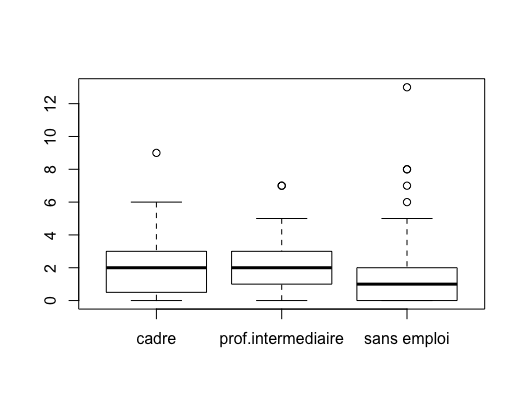
\includegraphics[scale=0.5]{ilu/lab5-1.png}\end{center}\end{figure}
> boxplot(n.enfant ~ prof, data=smpb,xlab="Profession", ylab="Nombre d'enfants",col="cornflowerblue", border="cornflowerblue")
> ##\begin{figure}[H]\begin{center}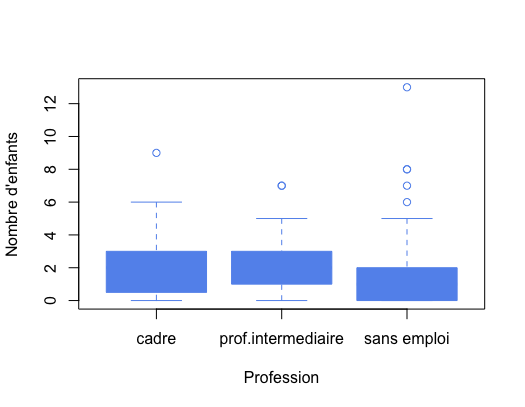
\includegraphics[scale=0.5]{ilu/lab5-2.png}\end{center}\end{figure}
> #############
> ##Nous allons a présent réaliser une ANOVA
> ###Recherche des informations sur la fonction Linear Model
> help(lm)
> lm(n.enfant ~ prof, data=smpb)

Call:
lm(formula = n.enfant ~ prof, data = smpb)

Coefficients:
           (Intercept)  profprof.intermediaire         profsans emploi  
               2.16667                -0.05952                -0.69718  

> ##Nous allons stocker le résultat de notre modèle de régression dans la variable m :
> m <- lm(n.enfant ~ prof, data=smpb)
> m

Call:
lm(formula = n.enfant ~ prof, data = smpb)

Coefficients:
           (Intercept)  profprof.intermediaire         profsans emploi  
               2.16667                -0.05952                -0.69718  

> ## Dans le cadre d'une ANOVA, nous allons utiliser la fonction qui en donnant le nom d'une variable et en spécifiant un test de Fisher Snedecor, de fournir un tableau d'analyse de variance,
> drop1(m,test = "F")
Single term deletions

Model:
n.enfant ~ prof
       Df Sum of Sq    RSS    AIC F value  Pr(>F)  
<none>              947.74 349.96                  
prof    2     25.05 972.79 353.60  3.8325 0.02276 *
---
Signif. codes:  0 '***' 0.001 '**' 0.01 '*' 0.05 '.' 0.1 ' ' 1
> ###Prof est la variable explicative
> ###2, le degré de liberté
> ### F value, correspondant à la valeur au test d'analyse de variance.
> ###=>la statistique de test 3.83 et ici le degré de significativité 0.02.
> ###Pour deux variables numériques :
> n <- lm(n.enfant ~ age, data=smpb)
> n

Call:
lm(formula = n.enfant ~ age, data = smpb)

Coefficients:
(Intercept)          age  
   -1.00902      0.06849  

> ##Intercept = ordonnée à l'origine
> ##age coef directeur
> ##Pour avoir les tests associés on tapera simplement summary(m) et on aura un tableau avec les coefficients de régression et les tests t associés ici pour la pente 10.77 et le degré de significativité.
> summary(n)

Call:
lm(formula = n.enfant ~ age, data = smpb)

Residuals:
    Min      1Q  Median      3Q     Max 
-4.2646 -0.9087 -0.2511  0.5708  9.0094 

Coefficients:
             Estimate Std. Error t value Pr(>|t|)    
(Intercept) -1.009022   0.262696  -3.841  0.00015 ***
age          0.068488   0.006357  10.773  < 2e-16 ***
---
Signif. codes:  0 '***' 0.001 '**' 0.01 '*' 0.05 '.' 0.1 ' ' 1

Residual standard error: 1.546 on 291 degrees of freedom
  (11 observations deleted due to missingness)
Multiple R-squared:  0.2851,  Adjusted R-squared:  0.2827 
F-statistic: 116.1 on 1 and 291 DF,  p-value: < 2.2e-16

> ##########################
> ##Depuis le début, nous travaillons sur un Data Frame Restreint que l'on a obtenu avec la fonction subset. La fonction lm() permet de réduire directement le Data Frame :
> ##On a donc juste à travailler avec le tableau d'origine et de définir les options de filtre que l'on souhaite appliquer :
> m<-lm(n.enfant ~ age,smp, subset =prof == "sans emploi" | prof == "prof.intermediaire" | prof == "cadre")
> summary(m)

Call:
lm(formula = n.enfant ~ age, data = smp, subset = prof == "sans emploi" | 
    prof == "prof.intermediaire" | prof == "cadre")

Residuals:
    Min      1Q  Median      3Q     Max 
-4.2646 -0.9087 -0.2511  0.5708  9.0094 

Coefficients:
             Estimate Std. Error t value Pr(>|t|)    
(Intercept) -1.009022   0.262696  -3.841  0.00015 ***
age          0.068488   0.006357  10.773  < 2e-16 ***
---
Signif. codes:  0 '***' 0.001 '**' 0.01 '*' 0.05 '.' 0.1 ' ' 1

Residual standard error: 1.546 on 291 degrees of freedom
  (17 observations deleted due to missingness)
Multiple R-squared:  0.2851,  Adjusted R-squared:  0.2827 
F-statistic: 116.1 on 1 and 291 DF,  p-value: < 2.2e-16

> ##On obtient donc les même valeurs
> ## l'intérêt ici, c'est que l'on peut utiliser à la fois une notation par formule, on décrit la relation entre le nombre d'enfants qui est la variable de réponse et l'âge qui est la variable explicative, ces variables se trouvent dans le data-frame qui s'appelle smp. Par contre ce data-frame-là va être filtré selon les critères qui sont indiqués (dans la commande) dans l'option subset.
> ############################################@
> ##On ne va s'intéresser qu'aux individus qui remplissent les conditions profession égal soit sans emploi, soit profession intermédiaire, soit cadre.
> ##Dès lors que l'on a un modèle de regression, on peut utiliser la commande coef pour afficher ces derniers :
> coef(m)
(Intercept)         age 
-1.00902159  0.06848829 
> coef(m)[1]
(Intercept) 
  -1.009022 
> coef(m)[2]
       age 
0.06848829 
> ##On peut utiliser pour obtenir les intervalles de confiance :
> confint(m)
                  2.5 %      97.5 %
(Intercept) -1.52604619 -0.49199700
age          0.05597581  0.08100076
> ##un tableau d'analyse de variance associé à la régression à l'aide de la commande anova() :
> anova(m)
Analysis of Variance Table

Response: n.enfant
           Df Sum Sq Mean Sq F value    Pr(>F)    
age         1 277.35  277.35  116.05 < 2.2e-16 ***
Residuals 291 695.44    2.39                      
---
Signif. codes:  0 '***' 0.001 '**' 0.01 '*' 0.05 '.' 0.1 ' ' 1
> ############################################
> ##Lorsque l'on souhaite réaliser des prédictions sur des valeurs non nécessairement observées on peut utiliser la commande predict().
> ###Dans ces cas-là on va lui donner le nom de la variable dans laquelle on a stocké notre modèle de régression et un data-frame dans lequel on va indiquer pour la variable qui sert de variable explicative les valeurs pour lesquelles on souhaite effectuer la prédiction.
> predict(m,data.frame(age=c(20,30,40)))
        1         2         3 
0.3607441 1.0456270 1.7305099 
> ##Si l'on souhaite déterminer en même temps les intervalles de confiances :
> predict(m,data.frame(age=c(20,30,40)),interval ="confidence" )
        fit        lwr       upr
1 0.3607441 0.06588459 0.6556037
2 1.0456270 0.83652266 1.2547313
3 1.7305099 1.55212966 1.9088901
> ##« fit » les valeurs prédites et « lwr », « upr » représentent les bornes inférieures et supérieures des intervalles de confiance à 95% pour la prévision.
> ############################################
> ##On peut également s'intéresser à la régression logisitique :
> ### On prend une varaible binaire (que l'on va construire) On va s'intéresser au nombre d'enfants supérieur à 2. Dans ces cas-là on codera 1 sinon on code 0
> smp$n.enfant.bin <- ifelse(smp$n.enfant > 2,1,0)
> table(smp$n.enfant)

  0   1   2   3   4   5   6   7   8   9  10  11  13 
214 220 125 101  55  31   7   7   7   2   2   1   1 
> table(smp$n.enfant.bin)

  0   1 
559 214 
> ##Pour effectuer une regression logisitique : c'est la commande glm() : Generalized Linear Models
> help(glm)
> m <- glm(n.enfant.bin ~ age , smp , family =binomial("logit"))
> summary(m)

Call:
glm(formula = n.enfant.bin ~ age, family = binomial("logit"), 
    data = smp)

Deviance Residuals: 
    Min       1Q   Median       3Q      Max  
-1.8551  -0.7525  -0.5326   0.8763   2.1301  

Coefficients:
             Estimate Std. Error z value Pr(>|z|)    
(Intercept) -3.827089   0.312803 -12.235   <2e-16 ***
age          0.069487   0.007016   9.904   <2e-16 ***
---
Signif. codes:  0 '***' 0.001 '**' 0.01 '*' 0.05 '.' 0.1 ' ' 1

(Dispersion parameter for binomial family taken to be 1)

    Null deviance: 912.06  on 772  degrees of freedom
Residual deviance: 794.16  on 771  degrees of freedom
  (26 observations deleted due to missingness)
AIC: 798.16

Number of Fisher Scoring iterations: 4

> ##cette fois-ci on a la variable explicative avec la valeur du coefficient de régression sur l'échelle du log odds.
> 
\end{lstlisting}
